\section{Classical estimates}\label{sec:classical}

\subsection{Method}

For each country, equation~\eqref{eq:okun} is estimated by ordinary least squares. Lag
orders are $K\in\{0,1,2,4\}$, with and without the change in the participation rate as a
control. The headline specification is $K=2$ without participation.

\paragraph{Inference.} Standard errors use the Newey--West covariance with a Bartlett
kernel and four lags in calendar quarters \citep{newey1987hac}. The variance of
$\hat\theta_i$ uses the full covariance matrix of the lag coefficients.

\paragraph{Samples.} The full period, 2009--2026; the same period without any observation
whose window touches 2020--2021; 2009--2019; 2022 onwards; and a flag-screened sample.

\paragraph{Review.} A separate review recomputed every published quantity by an
independent numerical route and re-estimated 24 core specifications per country. It
classified each country as robustly negative, negative with specification-dependent
significance, or sign-unstable.

\subsection{Results}

\paragraph{The association.} With 2020--2021 excluded, the two-lag sum is negative with a
95\% interval below zero in \val{cl_n_neg_excluded} of \val{n_countries} countries
(table~\ref{tab:countries}). In \val{cl_n_robust} countries every core specification agrees
in sign and excludes zero. These are associations conditional on contemporaneous and
lagged GDP growth. Contemporaneous growth is not exogenous, and the participation control
can absorb part of the association, a ``bad control'' in the sense of a variable that is
itself an outcome.

\paragraph{The pandemic.} Including 2020--2021 moves the sum towards zero in
\val{cl_n_attenuated} countries (figure~\ref{fig:pandemic}). In \val{cl_n_full_outside}
countries the full-sample estimate lies outside the 95\% interval of the estimate without
the pandemic. The pandemic quarters combine the largest output movements of the sample
with job-retention schemes that kept unemployment from following output. The full-sample
coefficient therefore describes those quarters, not the 2009--2019 relationship.

\paragraph{Post-2021 stability.} The original classical analysis tested whether the sum
changed after 2021 with interacted HAC regressions and Holm's step-down adjustment
\citep{holm1979}; \val{ss_published_holm} changes were significant. With only about
seventeen post-2021 quarters, however, the asymptotic normal reference is unreliable. A
pre-registered study replaced it with null-imposed sieve and moving-block bootstraps of the
same statistic \citep{kunsch1989bootstrap}:
\begin{itemize}
  \item \val{ss_survivors} of the \val{ss_published_holm} published changes survive;
  \item a size study under each test's fitted null shows why: the nominal 5\% normal test
    rejects \val{ss_size_normal} of the time, whereas the bootstrap test rejects
    \val{ss_size_bootstrap}.
\end{itemize}
A weaker association after 2021 is therefore a descriptive pattern, not a tested result.
The Bayesian regime models (section~\ref{sec:bayes}) agree.

% Generated by eu-okun publication. Do not edit.
\begin{table}[htbp]\centering\small
\caption{Two-lag sums $\theta_i=\sum_{k=0}^{2}\beta_{ik}$ (pp of unemployment-rate change per pp of quarterly GDP growth). Classical: OLS on the full sample and without 2020--2021; the interval is the small-sample bootstrap-$t$ 95\% interval of the Newey--West statistic (normal intervals over-reject with this few quarters). $^{*}$ significantly negative under both registered bootstraps; $^{**}$ also after the registered Holm adjustment. Bayesian: posterior median and 90\% credible interval of the primary hierarchical model (2009--2019). Verdict over the core grid without the participation control (normal intervals): robust negative (robust), negative with specification-dependent significance (spec.-dep.), or sign-unstable. Alphabetical; no ranking is implied. Descriptive associations. The original review, which also counted participation-controlled specifications, classed RO as spec.-dep.}
\label{tab:countries}
\begin{tabular}{lrrrl}
\toprule
Country & Full sample & Without 2020--21 [bootstrap 95\%] & Bayes median [90\%] & Verdict \\
\midrule
AT & $-0.23$ & $-0.21^{*}$ $[-0.37, -0.05]$ & $-0.18$ $[-0.30, -0.07]$ & robust \\
BE & $-0.03$ & $-0.14$ $[-0.75, +0.45]$ & $-0.24$ $[-0.40, -0.08]$ & spec.-dep. \\
BG & $-0.33$ & $-0.41^{*}$ $[-0.69, -0.14]$ & $-0.17$ $[-0.31, -0.03]$ & robust \\
CY & $-0.27$ & $-0.47^{*}$ $[-0.68, -0.26]$ & $-0.25$ $[-0.36, -0.13]$ & robust \\
CZ & $-0.19$ & $-0.27^{*}$ $[-0.38, -0.17]$ & $-0.17$ $[-0.24, -0.09]$ & robust \\
DE & $-0.10$ & $-0.18^{*}$ $[-0.30, -0.05]$ & $-0.11$ $[-0.18, -0.05]$ & robust \\
DK & $-0.18$ & $-0.14$ $[-0.53, +0.24]$ & $-0.19$ $[-0.31, -0.07]$ & spec.-dep. \\
EE & $-0.46$ & $-0.49^{**}$ $[-0.71, -0.28]$ & $-0.32$ $[-0.47, -0.18]$ & robust \\
EL & $-0.40$ & $-0.62^{*}$ $[-0.84, -0.40]$ & $-0.37$ $[-0.48, -0.23]$ & robust \\
\textbf{ES} & $-0.27$ & $-0.79^{*}$ $[-1.15, -0.45]$ & $-0.51$ $[-0.67, -0.30]$ & robust \\
FI & $-0.28$ & $-0.24^{*}$ $[-0.36, -0.12]$ & $-0.20$ $[-0.30, -0.10]$ & robust \\
FR & $-0.00$ & $-0.30^{*}$ $[-0.49, -0.12]$ & $-0.20$ $[-0.30, -0.10]$ & sign-unstable \\
HR & $-0.16$ & $-0.47^{*}$ $[-0.84, -0.09]$ & $-0.27$ $[-0.44, -0.12]$ & spec.-dep. \\
HU & $-0.13$ & $-0.18^{*}$ $[-0.30, -0.06]$ & $-0.16$ $[-0.25, -0.06]$ & robust \\
IE & $-0.06$ & $-0.07^{*}$ $[-0.13, +0.00]$ & $-0.06$ $[-0.11, -0.02]$ & robust \\
IT & $-0.04$ & $-0.51^{*}$ $[-0.80, -0.22]$ & $-0.32$ $[-0.50, -0.15]$ & spec.-dep. \\
LT & $-0.36$ & $-0.45^{*}$ $[-0.81, -0.08]$ & $-0.24$ $[-0.36, -0.11]$ & robust \\
\textbf{LU} & $-0.05$ & $+0.17$ $[-0.06, +0.40]$ & $-0.11$ $[-0.23, +0.01]$ & sign-unstable \\
LV & $-0.32$ & $-0.37$ $[-0.81, +0.08]$ & $-0.27$ $[-0.38, -0.14]$ & robust \\
MT & $-0.09$ & $-0.01$ $[-0.07, +0.04]$ & $-0.04$ $[-0.09, +0.00]$ & spec.-dep. \\
\textbf{NL} & $-0.21$ & $-0.28^{*}$ $[-0.51, -0.05]$ & $-0.13$ $[-0.23, -0.04]$ & robust \\
PL & $-0.09$ & $-0.24^{*}$ $[-0.40, -0.08]$ & $-0.13$ $[-0.21, -0.06]$ & robust \\
\textbf{PT} & $-0.13$ & $-0.49^{*}$ $[-0.82, -0.18]$ & $-0.25$ $[-0.39, -0.12]$ & spec.-dep. \\
RO & $-0.11$ & $-0.07$ $[-0.15, +0.02]$ & $-0.05$ $[-0.09, -0.00]$ & robust \\
SE & $-0.22$ & $-0.22^{*}$ $[-0.41, -0.02]$ & $-0.17$ $[-0.25, -0.11]$ & robust \\
SI & $-0.18$ & $-0.25^{*}$ $[-0.47, -0.02]$ & $-0.15$ $[-0.26, -0.04]$ & robust \\
SK & $-0.13$ & $+0.04$ $[-0.85, +0.91]$ & $-0.09$ $[-0.20, +0.01]$ & sign-unstable \\
\bottomrule
\end{tabular}
\end{table}


\begin{figure}[t]\centering
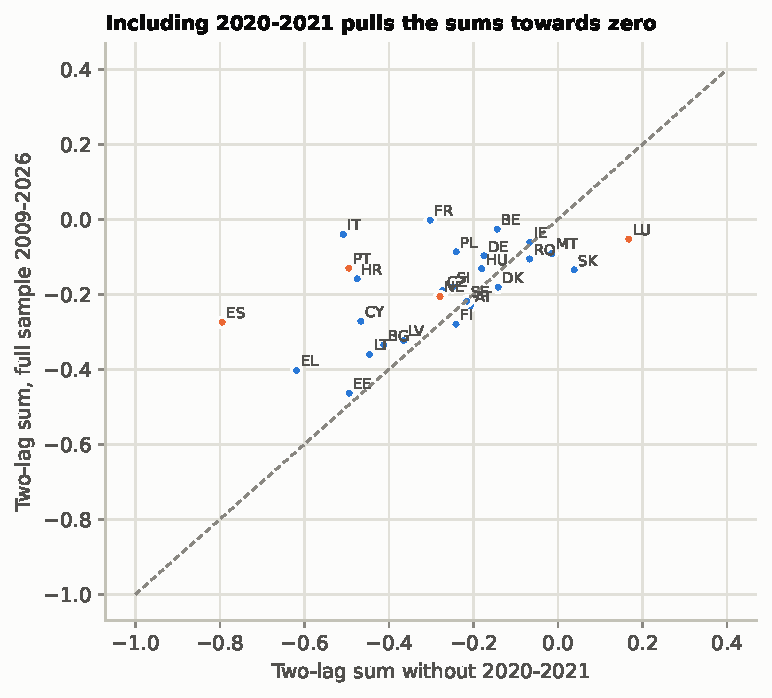
\includegraphics[width=0.62\textwidth]{fig2_pandemic.pdf}
\caption{Classical two-lag sums ($K=2$): full sample (vertical) against the sample without
2020--2021 (horizontal). For negative sums, a point above the diagonal is closer to zero
when the pandemic quarters are included. Focus countries in orange.}\label{fig:pandemic}
\end{figure}
